%% Auteur: Simon-Pierre Boucher, Université Laval, Chapitre 2 : thèse de doctorat

\section{Figures}


\begin{landscape}
\begin{figure}[t]
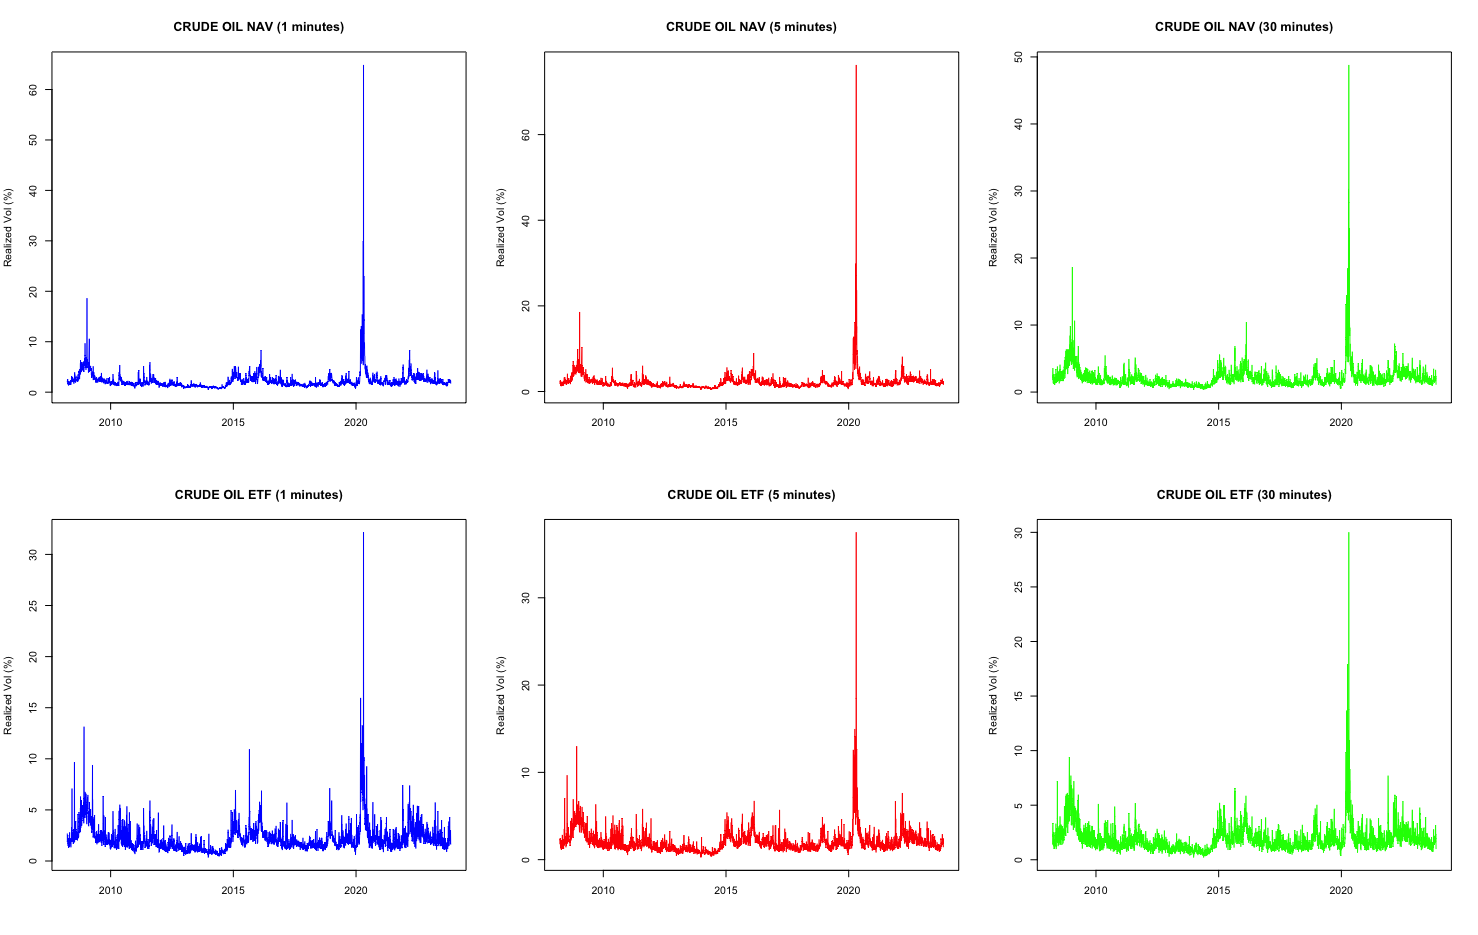
\includegraphics[width=16cm]{USO.png}
\centering
\caption{Realized Volatility for Crude Oil (ETF and NAV)}
\label{fig:rv_uso}
\end{figure}
\end{landscape}

\begin{landscape}
\begin{figure}[t]
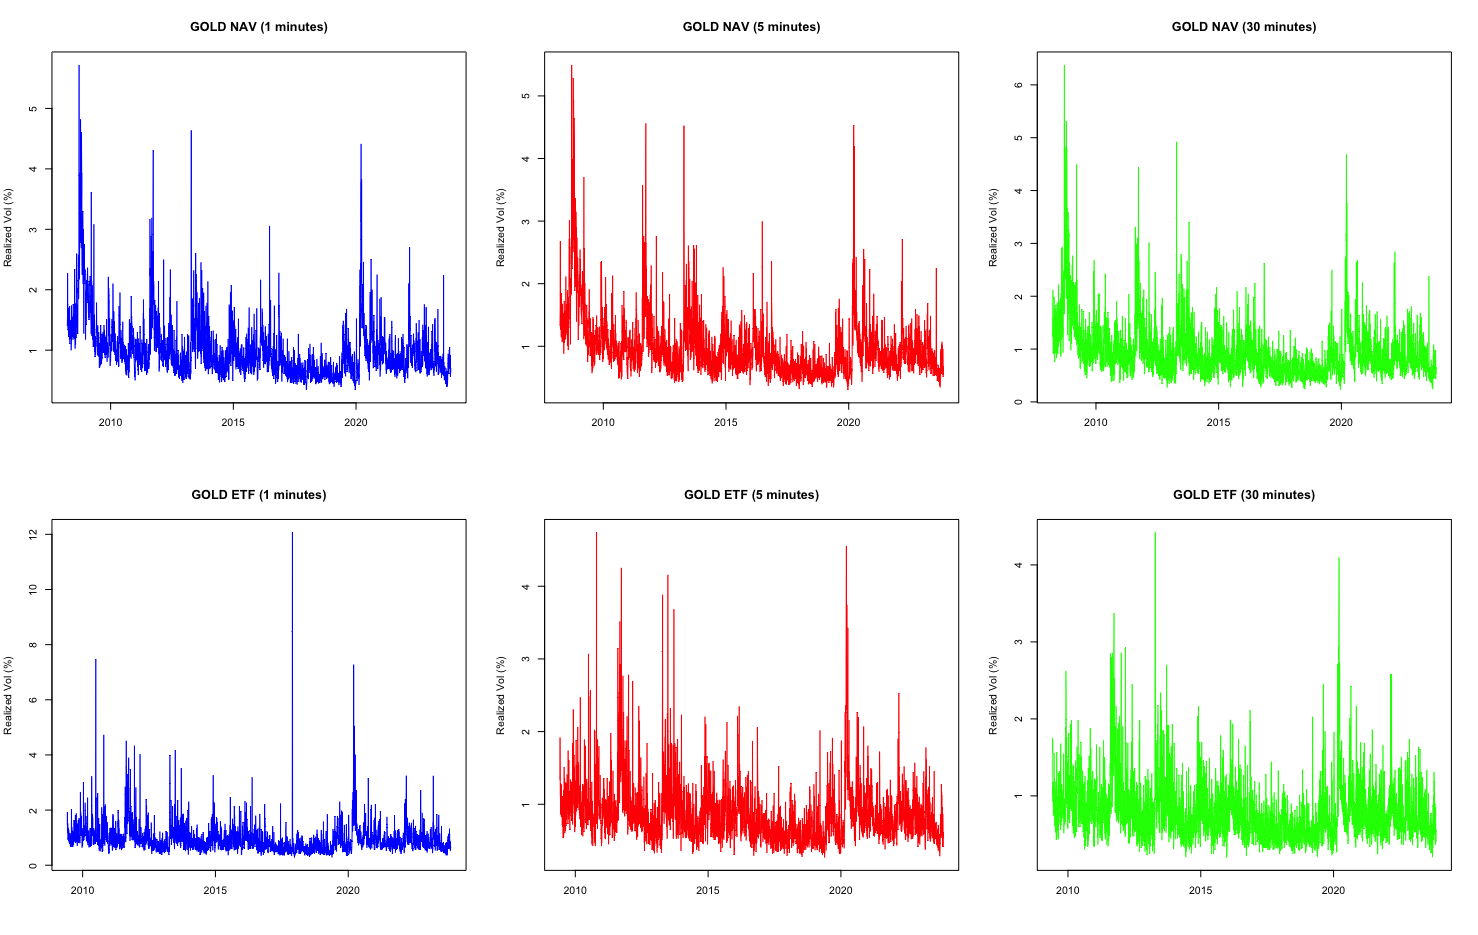
\includegraphics[width=16cm]{GLD.png}
\centering
\caption{Realized Volatility for Gold (ETF and NAV)}
\label{fig:rv_gld}
\end{figure}
\end{landscape}

\begin{landscape}
\begin{figure}[t]
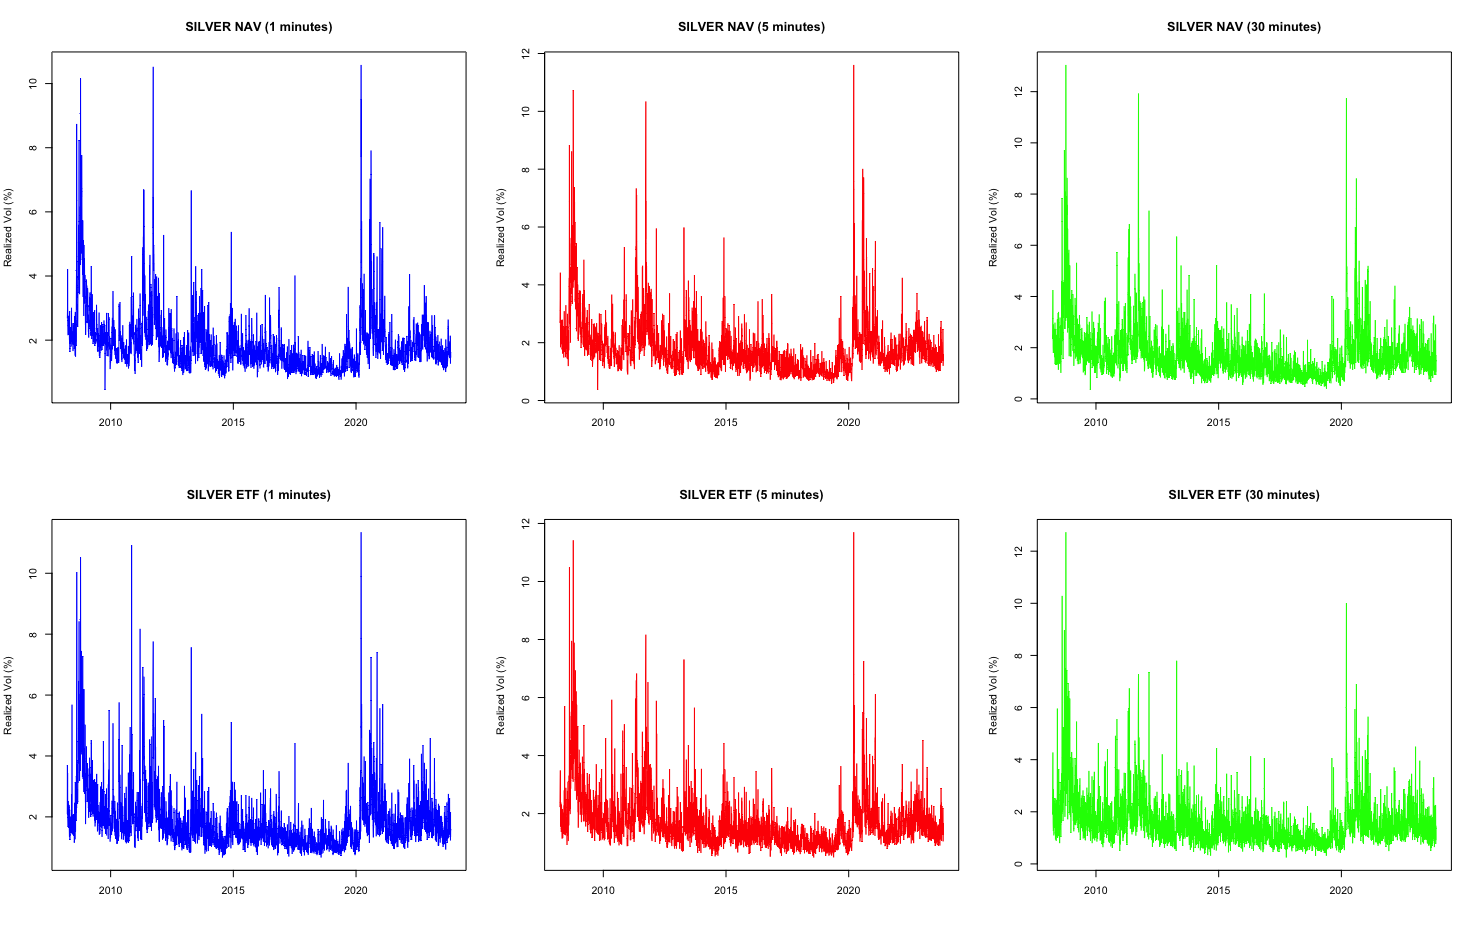
\includegraphics[width=16cm]{SLV.png}
\centering
\caption{Realized Volatility for Silver (ETF and NAV)}
\label{fig:rv_slv}
\end{figure}
\end{landscape}

\begin{landscape}
\begin{figure}[t]
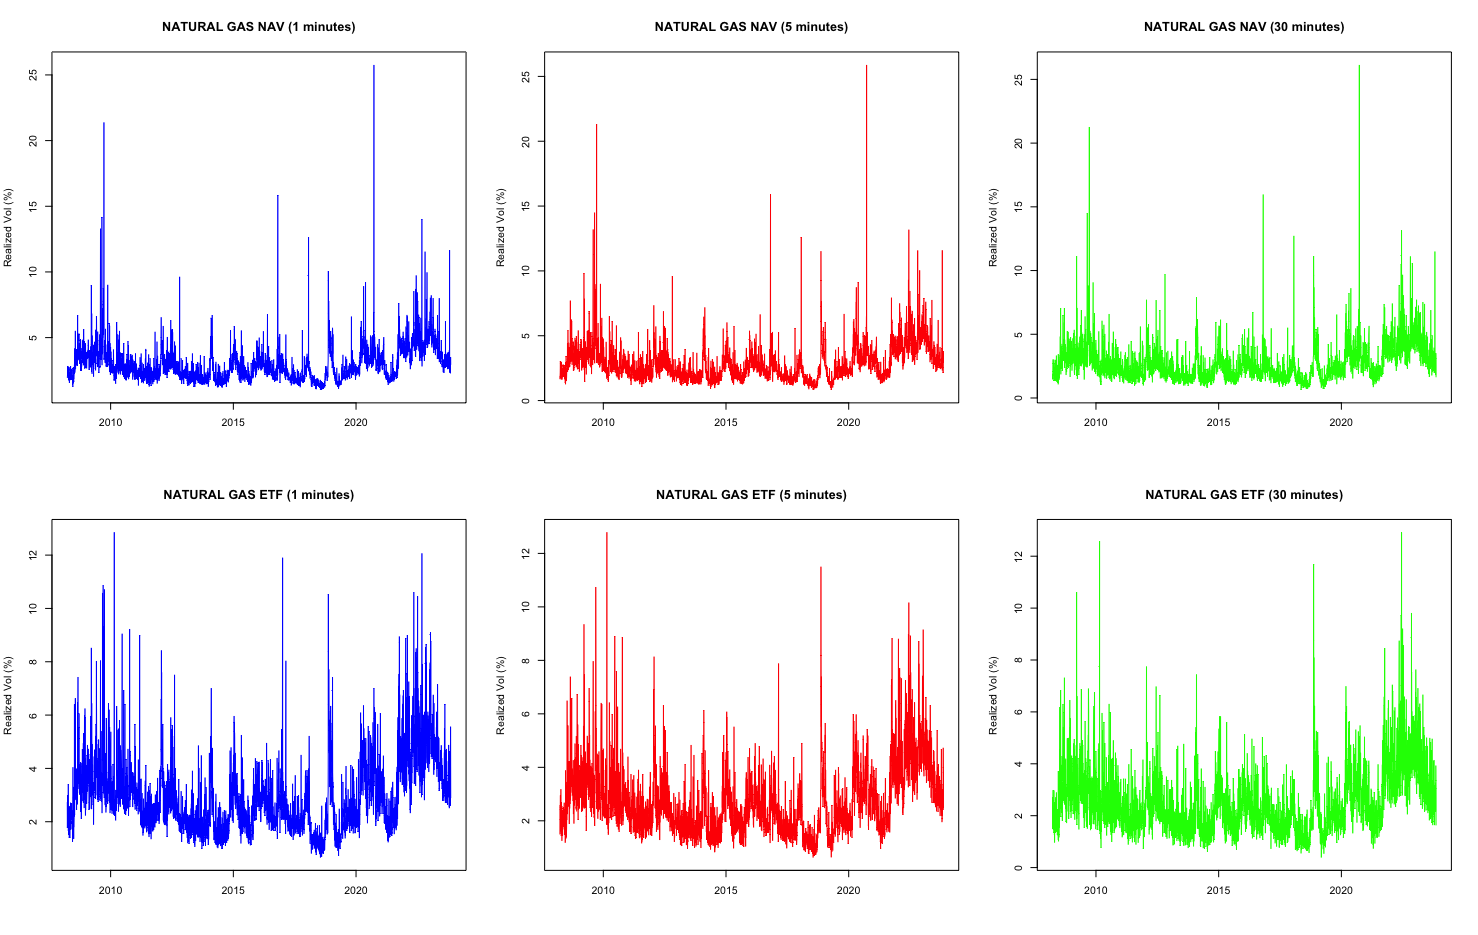
\includegraphics[width=16cm]{UNG.png}
\centering
\caption{Realized Volatility for Natural Gas (ETF and NAV)}
\label{fig:rv_ung}
\end{figure}
\end{landscape}

\begin{landscape}
\begin{figure}[t]
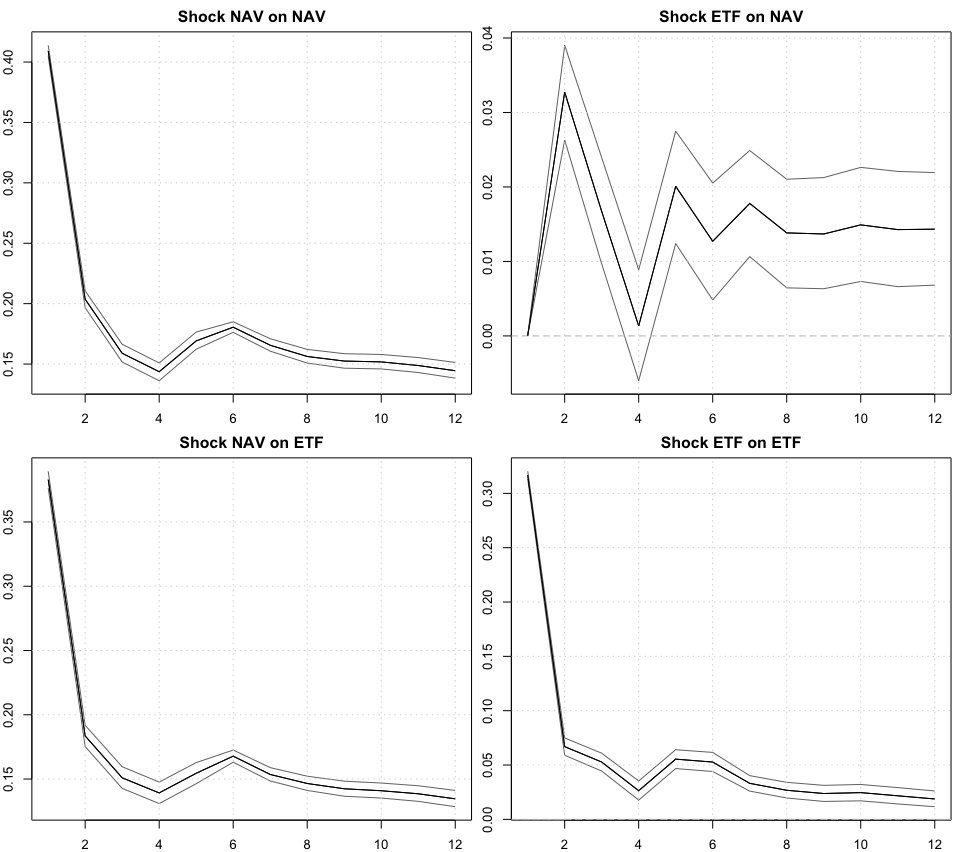
\includegraphics[width=16cm]{USO_irf.png}
\centering
\caption{Impulse Response Function (IRF) resulting from the modeling of the USO ETF and its Net Asset Value (NAV)}
\label{fig:irf1}
\end{figure}
\end{landscape}

\begin{landscape}
\begin{figure}[t]
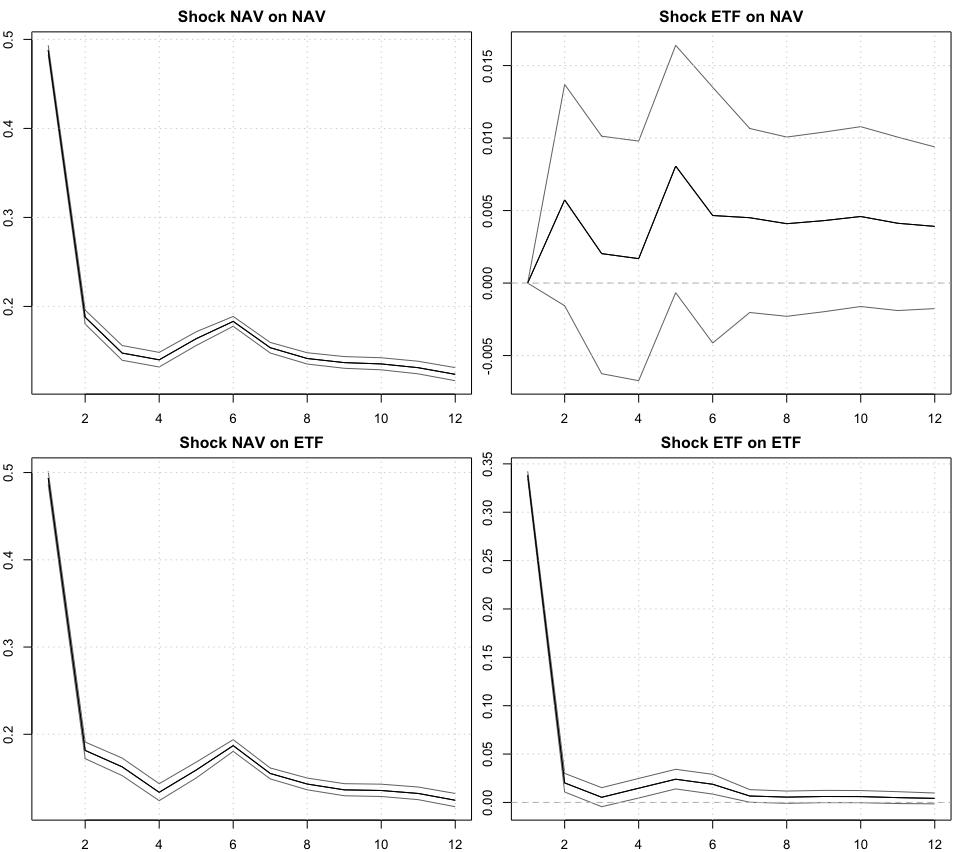
\includegraphics[width=16cm]{GLD_irf.png}
\centering
\caption{Impulse Response Function (IRF) resulting from the modeling of the GLD ETF and its Net Asset Value (NAV)}
\label{fig:irf2}
\end{figure}
\end{landscape}

\begin{landscape}
\begin{figure}[t]
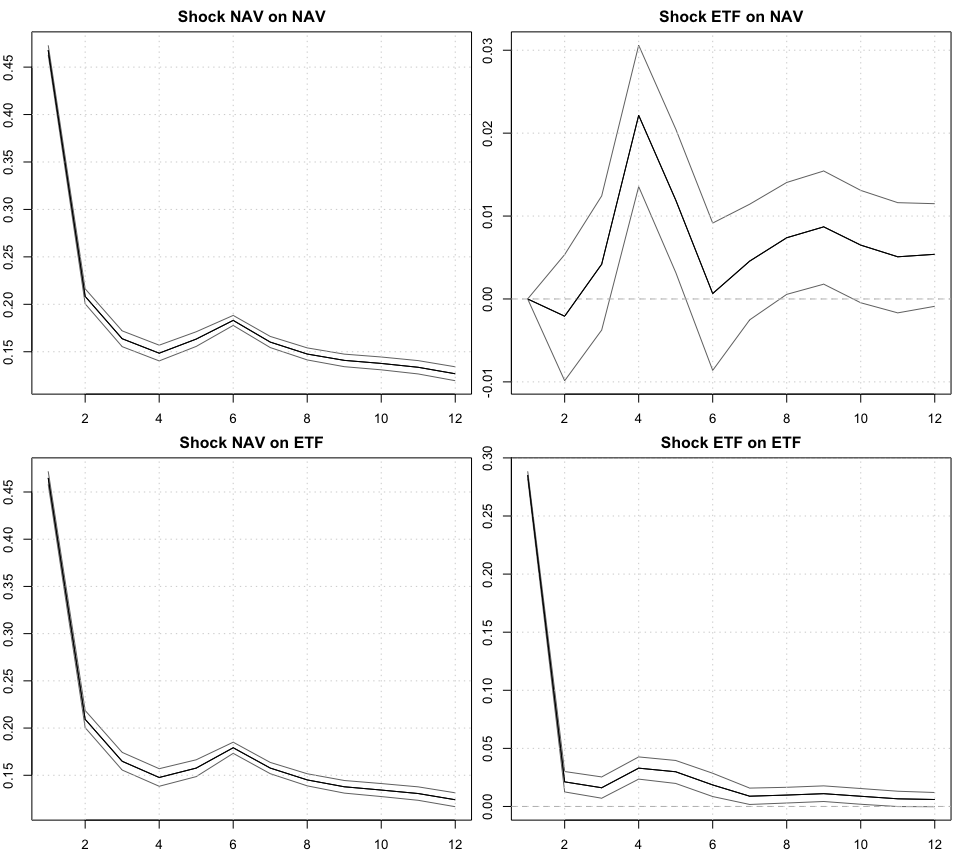
\includegraphics[width=16cm]{SLV_irf.png}
\centering
\caption{Impulse Response Function (IRF) resulting from the modeling of the SLV ETF and its Net Asset Value (NAV)}
\label{fig:irf3}
\end{figure}
\end{landscape}

\begin{landscape}
\begin{figure}[t]
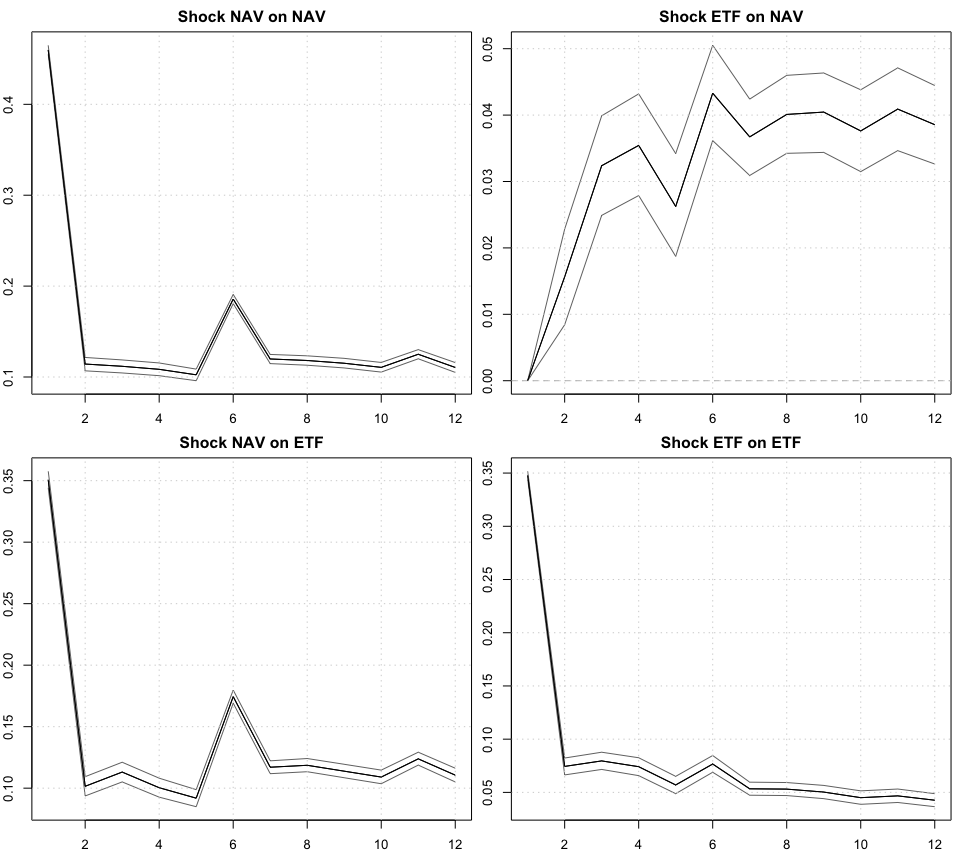
\includegraphics[width=16cm]{UNG_irf.png}
\centering
\caption{Impulse Response Function (IRF) resulting from the modeling of the UNG ETF and its Net Asset Value (NAV)}
\label{fig:irf4}
\end{figure}
\end{landscape}
